\documentclass[10pt,a4paper]{exam}
\usepackage[utf8]{inputenc}
\usepackage{amsmath}
\usepackage{amsfonts}
\usepackage{bbm}
\usepackage{commath}
\usepackage{amssymb}
\usepackage{booktabs}
\usepackage{blkarray}
\usepackage{systeme}
\usepackage{graphicx}
\usepackage[left=.75in,right=.75in,top=.75in,bottom=.75in]{geometry}

\usepackage{tikz}
\usetikzlibrary{chains}
\printanswers


\author{Ryan Honea}
\title{Time Series Analysis Homework 4}
\begin{document}
\begin{center}
Time Series Homework 4\\
Ryan Honea
\end{center}
\begin{questions}
\question Download data sets from D2L. For each data sets plot the ACF and ACVF. Using those plot guess appropriate time series model/models, also provide explanation to support your choice. Maximum two guesses are allowed.
\begin{parts}
\part Data-1
\begin{solution}
Based on the initial data plot which shows stationarity, we can do traditional analysis of the ACF and PACF plots.
\begin{center}
\includegraphics[scale=.4]{data1}
\end{center}
\begin{center}
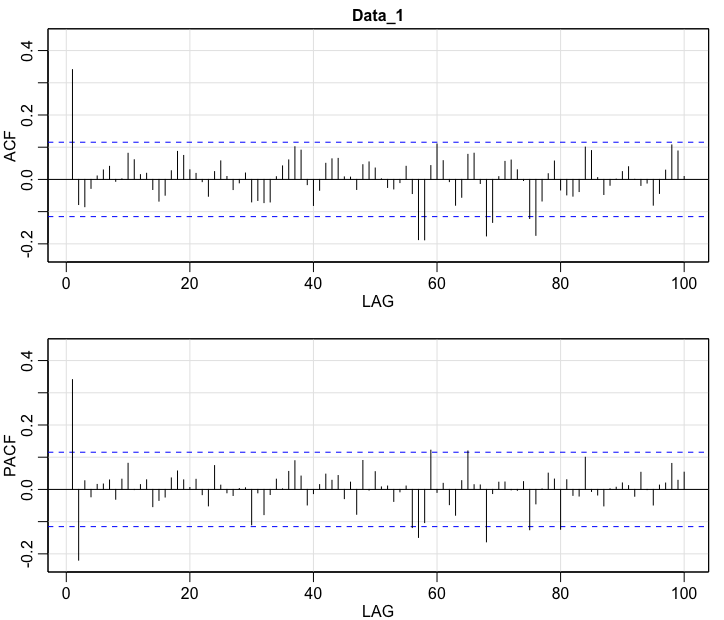
\includegraphics[width=.9\linewidth]{data1plot}
\end{center}
Based on the diminishing result in the ACF plot after lag 1, and the diminishing result in the PACF plot after lag 2, I'd argue that the model is $ARMA(2,1)$. I could also potentially see it being $AR(2)$.
\end{solution}

\part Data-2
\begin{solution}
Based on the initial data plot which shows stationarity, we can do traditional analysis of the ACF and PACF plots.
\begin{center}
\includegraphics[scale=.4]{data2}
\end{center}
\begin{center}
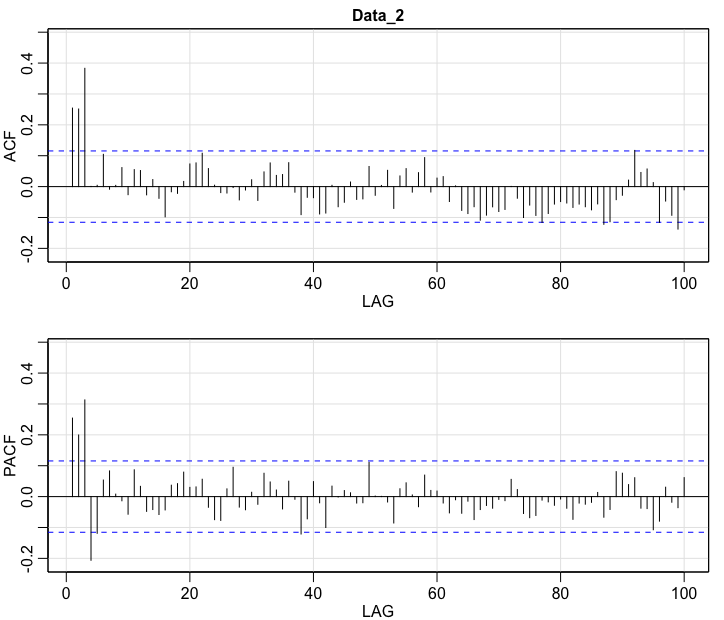
\includegraphics[width=.9\linewidth]{data2plot}
\end{center}
Based on the plots significant lags, with logic similar to on Data-1, I'd argue that the data is $Arma(5,3)$. However, the significant results in the ACF plot could be due to the AR process and so my second guess would be $AR(5)$.
\end{solution}
\pagebreak

\part Data-3
\begin{solution}
The initial data plot is not clearly stationary, but with an ADF test with p-value .01, we assume stationarity and so traditional analysis of ACF and PACF plots is appropriate..
\begin{center}
\includegraphics[scale=.4]{data3}
\end{center}
\begin{center}
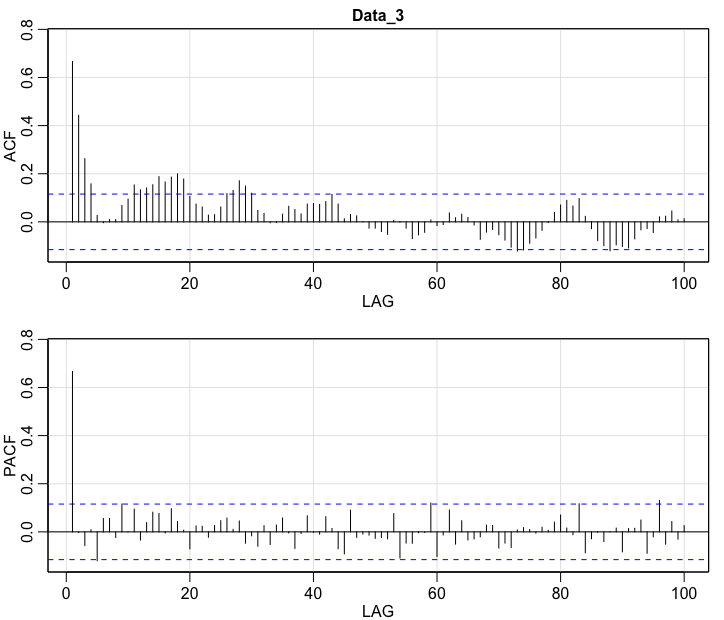
\includegraphics[width=.9\linewidth]{data3plot}
\end{center}
Since the ACF seems to be changing pretty geometrically for the most part and the PACF only jumps at 1, I'd say this is an $AR(1)$ process. It could potentially be $AR(1,1)$.
\end{solution}
\pagebreak

\part Data-4
\begin{solution}
The initial plot is clearly not stationarity and this is verified by an ADF test, so we difference it once and achieve stationarity.
\begin{center}
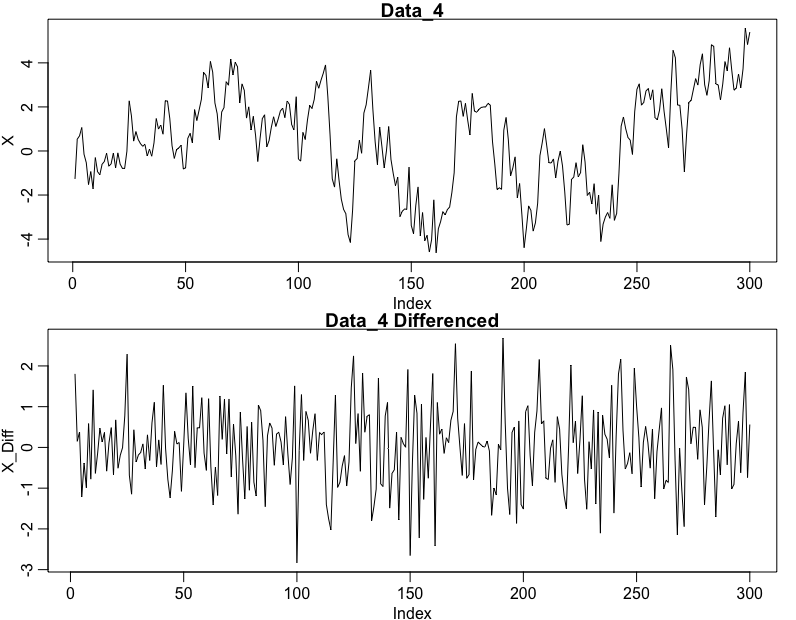
\includegraphics[scale=.4]{data4}
\end{center}
\begin{center}
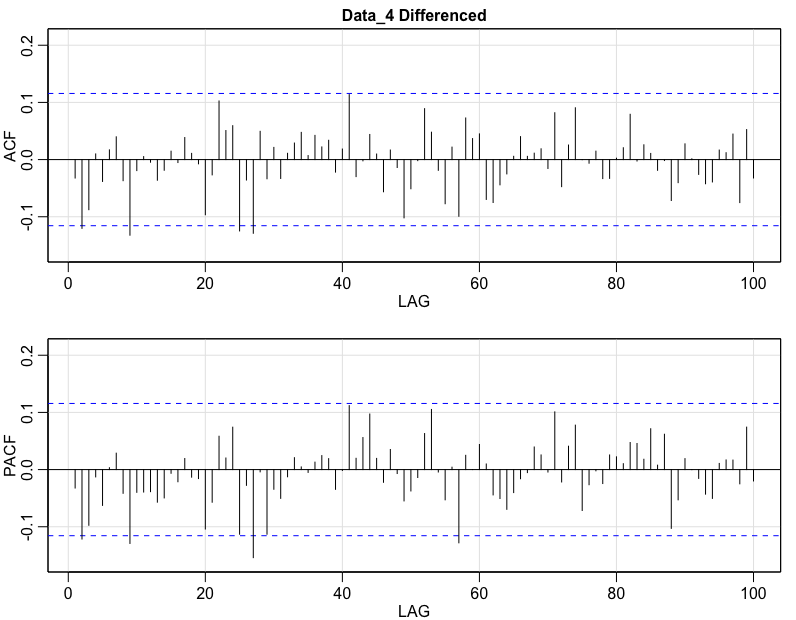
\includegraphics[width=.9\linewidth]{data4plot}
\end{center}
This doesn't appear to have any autocorrelation or partial autocorrelation, so perhaps the data is $ARIMA(1,1,0)$. Another guess is $ARIMA(1,0,1)$.
\end{solution}
\pagebreak

\part Data-5
\begin{solution}
The initial plot is not obviously stationary but an ADF test on the data shows that it likely is. So traditional analysis should work.
\begin{center}
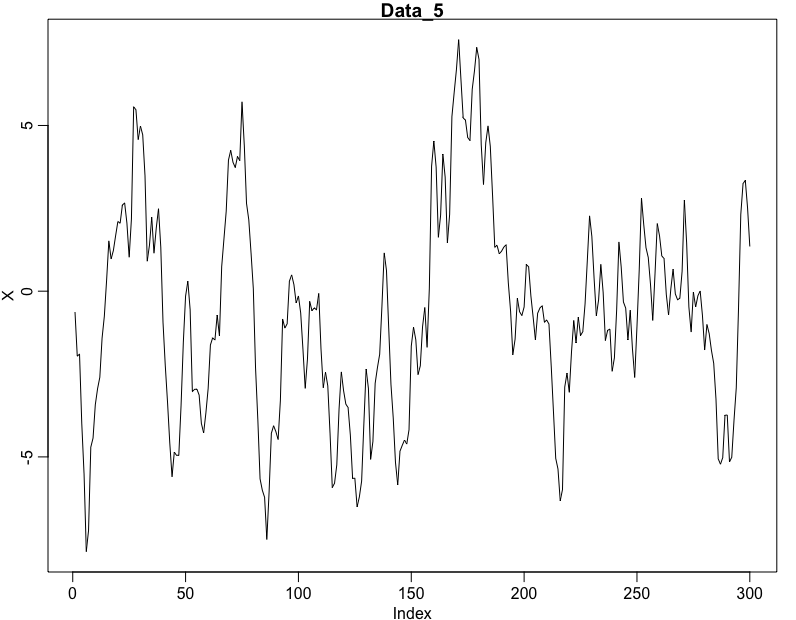
\includegraphics[scale=.4]{data5}
\end{center}
\begin{center}
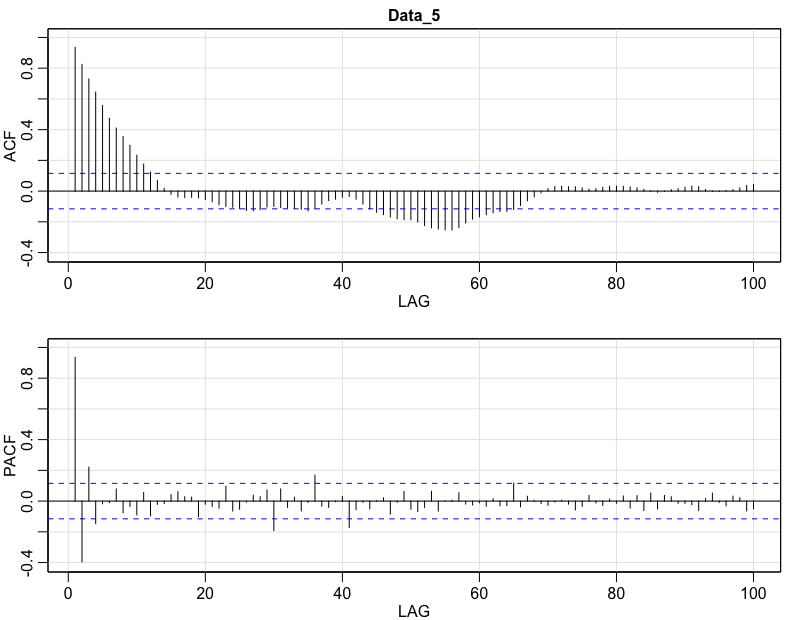
\includegraphics[width=.9\linewidth]{data5plot}
\end{center}
Based on the nearly geometric progression of the ACF, I would say that most of the effect comes from an $AR(4)$ process based on the PACF.
\end{solution}

\pagebreak
\part Data-6
\begin{solution}
Without even testing, it's clear that this model is not stationary and needs differencing.
\begin{center}
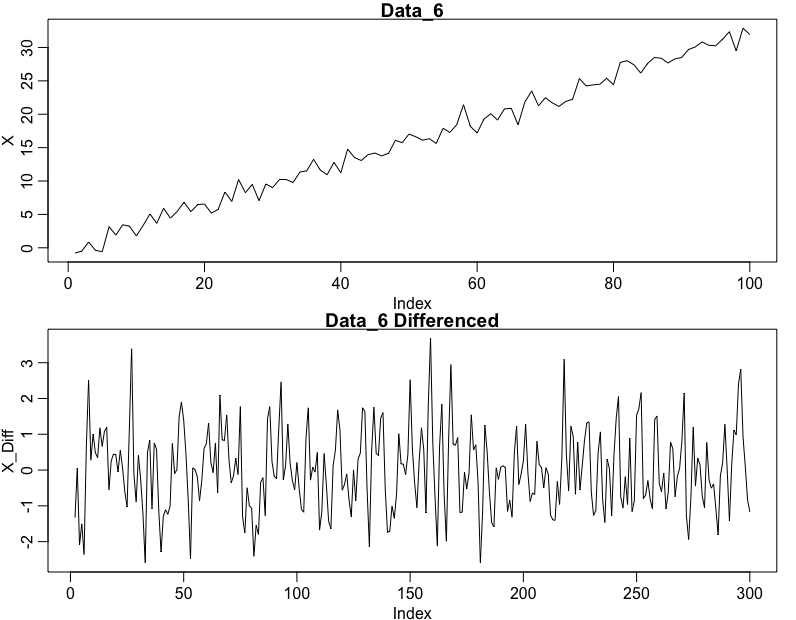
\includegraphics[scale=.4]{data6}
\end{center}
\begin{center}
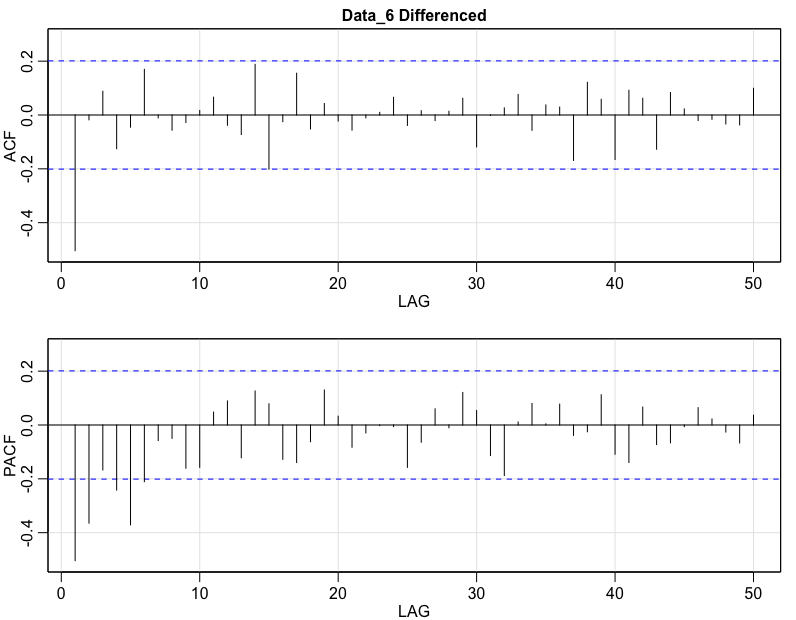
\includegraphics[width=.9\linewidth]{data6plot}
\end{center}
Based on these plots, I would say that this is $ARIMA(5,1,1)$ or maybe $ARIMA(2,1,1)$. \end{solution}
\pagebreak

\part Data-7
\begin{solution}
The initial plot shows stationarity and is verified by an ADF test with p-value less than .01. So analysis of the plots should be sufficient.
\begin{center}
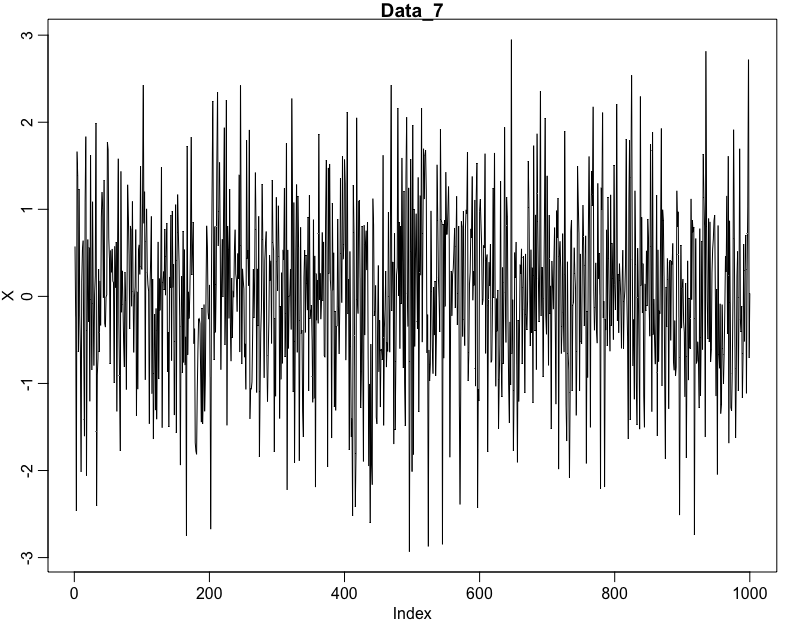
\includegraphics[scale=.4]{data7}
\end{center}
\begin{center}
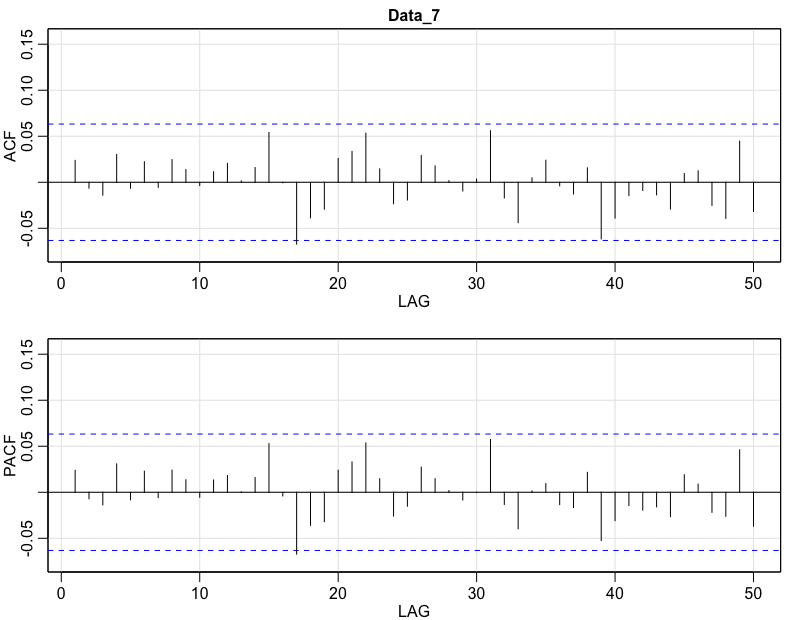
\includegraphics[width=.9\linewidth]{data7plot}
\end{center}
This is just white noise based on these plots.
\end{solution}
\pagebreak

\part Data-8
\begin{solution}
The data appears stationary and ADF test verifies this.
\begin{center}
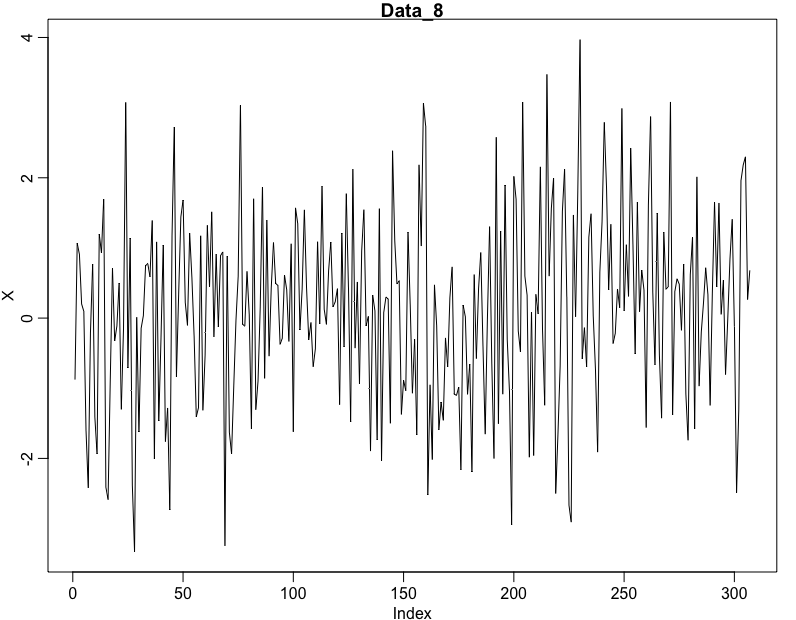
\includegraphics[scale=.4]{data8}
\end{center}
\begin{center}
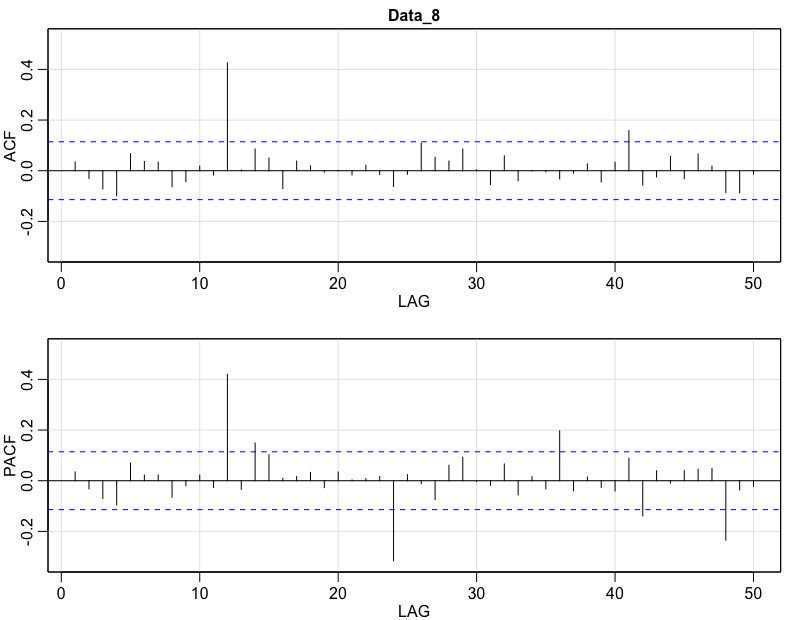
\includegraphics[width=.9\linewidth]{data8plot}
\end{center}
Based on the jumps in ACF and PACF at lag 12, this is definitely seasonal. This is perhaps $ARMA(0,0)\times (2,1)_{d=12}$ or perhaps $ARMA(0,0)\times (2,0)_{d=12}$.
\end{solution}
\pagebreak

\part Data-9
\begin{solution}
The data is clearly stationary, but an ADF verifies that it likely is.
\begin{center}
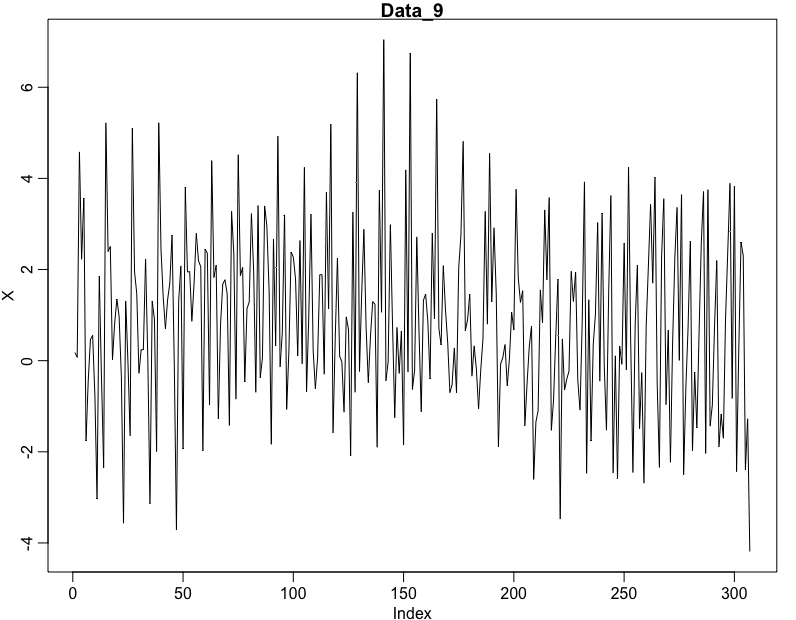
\includegraphics[scale=.4]{data9}
\end{center}
\begin{center}
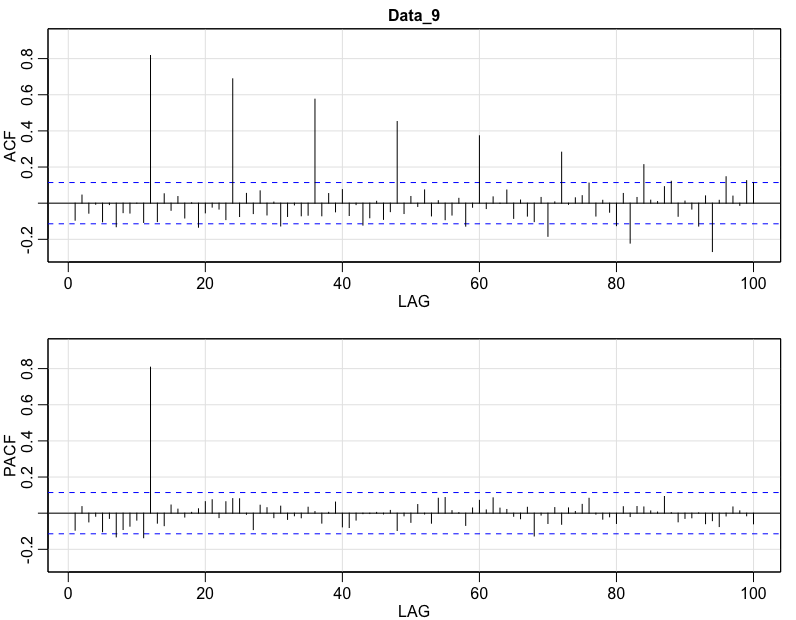
\includegraphics[width=.9\linewidth]{data9plot}
\end{center}
This one isn't so easy, but I would argue that most of the MA effect comes from the seasonal effect within the AR part of the process. I think this could be $ARMA(0,0)\times (1,1)_{d=12}$ or maybe the MA could be dropped leaving just $ARMA(0,0)\times(1,0)_{d=12}$.\end{solution}

\pagebreak
\part Data-10
\begin{solution}
Wildly enough, while the plot appears to not be stationary, an ADF test argues that it is. I will believe it, but highly doubt it.
\begin{center}
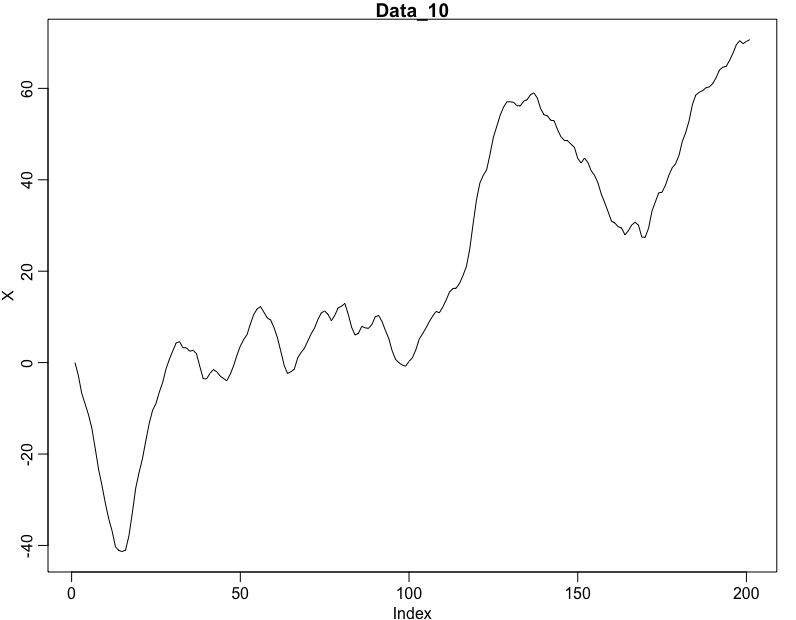
\includegraphics[scale=.4]{data10}
\end{center}
\begin{center}
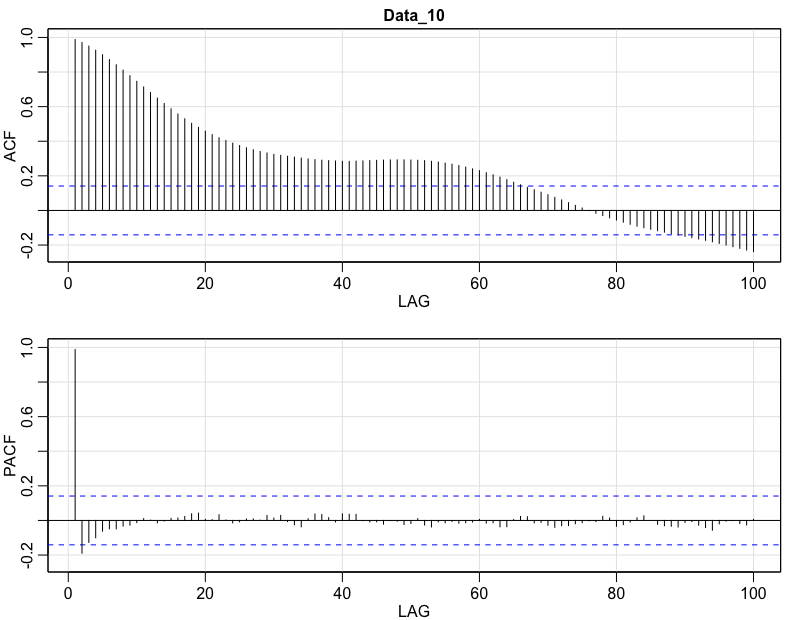
\includegraphics[width=.9\linewidth]{data10plot}
\end{center}
The best I can come up with this strange plot is $AR(2)$ or maybe $AR(2,1)$. The MA effects could be mostly from the AR effect, but this is not decreasing geometrically which is why the effect from an MA process might be necessary.
\end{solution}
\end{parts}
\pagebreak



\question Use the ``AirPassenger" data and fit a linear, quadratic, and cubic trend and for each trend you fit plot the residuals. Extract trend seasonality using non parametric methods. Provide R code and the plots.

\begin{solution}
Using the below code, graphs are obtained.
\begin{verbatim}
fit1 <- tslm(AirPassengers ~ trend)
fit2 <- tslm(AirPassengers ~ poly(trend,2))
fit3 <- tslm(AirPassengers ~ poly(trend,3))
par(mfrow = c(1,3))
plot.ts(AirPassengers, main = "Linear", cex.main=1.5)
lines(fitted(fit1), lwd=2, col=2, lty = 2)
plot.ts(AirPassengers, main = "Quadratic", cex.main=1.5)
lines(fitted(fit2), lwd=2, col=2, lty = 2)
plot.ts(AirPassengers, main = "Cubic", cex.main=1.5)
lines(fitted(fit3), lwd=2, col=2, lty = 2)

plot(fit1$residuals, main = "Linear")
plot(fit2$residuals, main = "Quadratic")
plot(fit3$residuals, main = "Cubic")
\end{verbatim}

\begin{center}
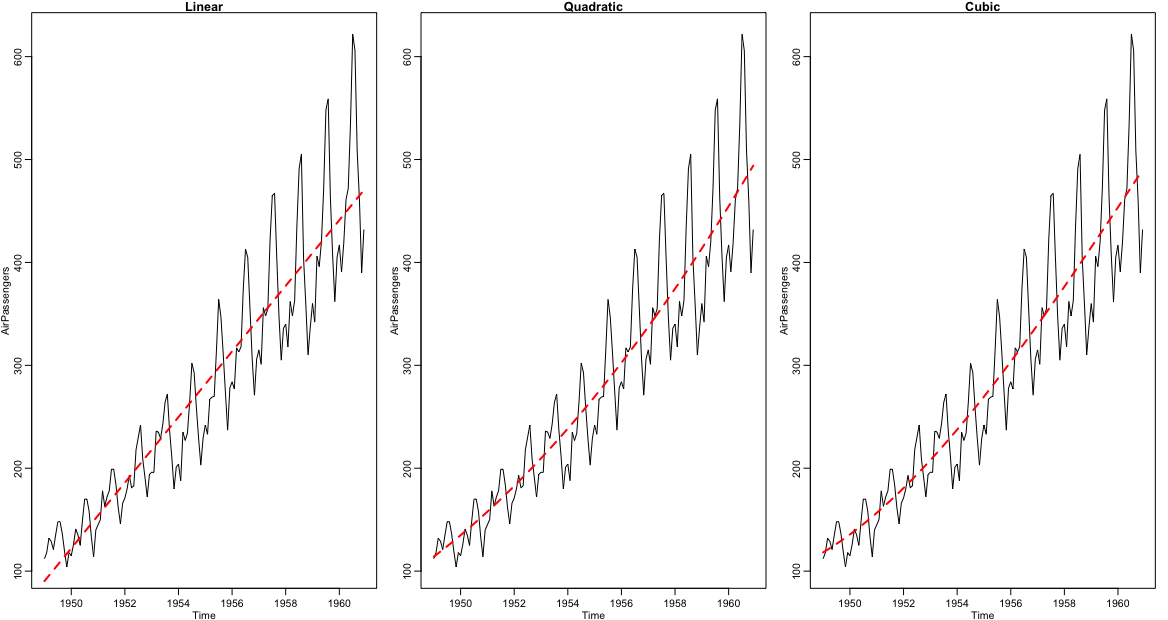
\includegraphics[width=.9\linewidth]{AirPassengersFits}
\end{center}


\begin{center}
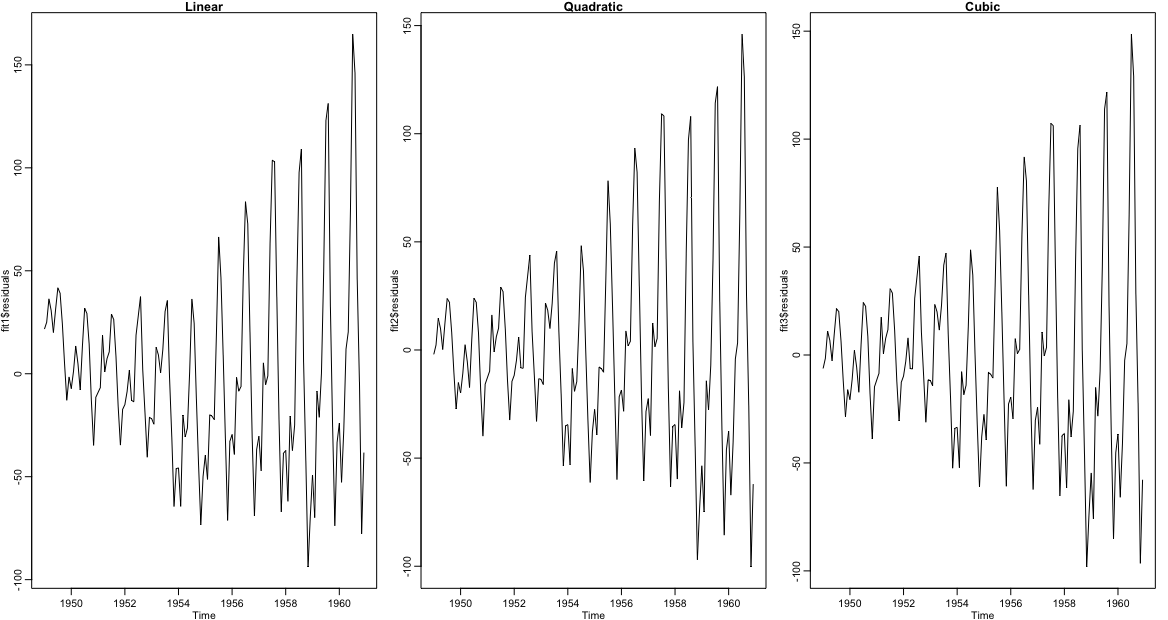
\includegraphics[width=.9\linewidth]{AirPassengerResiduals}
\end{center}
\end{solution}
\pagebreak
\begin{solution}
We can extract the seasonality by decomposition and use of a periodogram. I utilize the Additive and Multiplicative nonparametric methods to extract seasonality and that is done below.
\begin{verbatim}
data(AirPassengers)
xt=AirPassengers
par(mfrow=c(1,2))

#Additive Effect
decomp.x.ad=decompose(xt,type = "additive")
periodogram(decomp.x.ad$seasonal, main = "Additive")

#Multiplicative Effect
decomp.x.mul=decompose(xt,type = "multiplicative")
periodogram(decomp.x.mul$seasonal, main = "Multiplicative")
\end{verbatim}

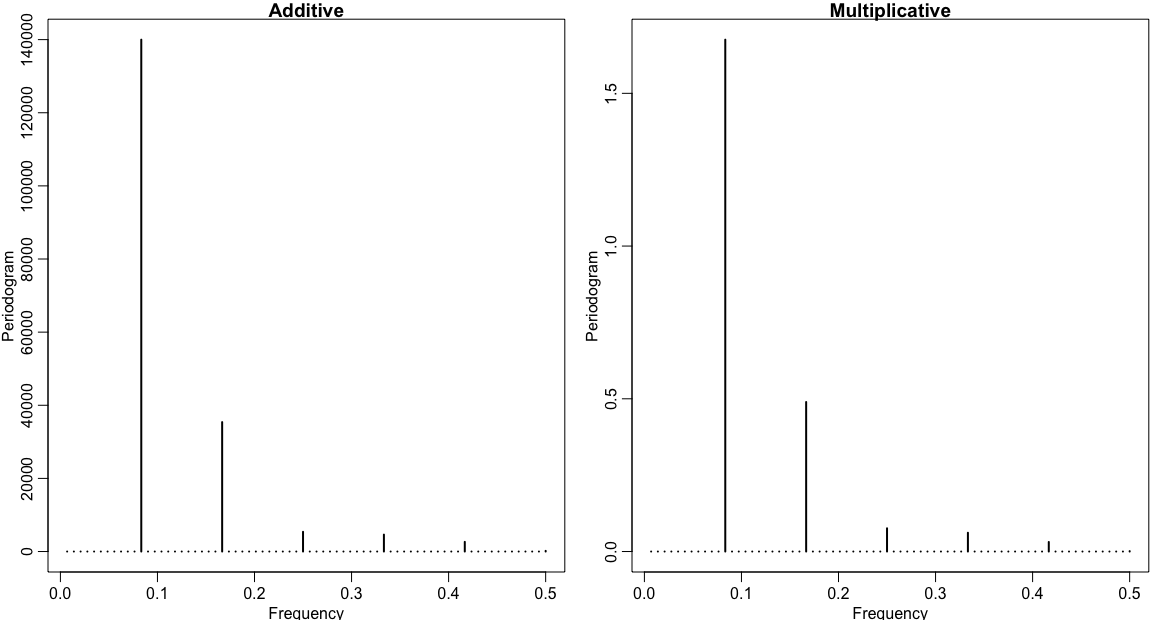
\includegraphics[width=.9\linewidth]{AirPassengerSeasonality}


The highest peak appears to be around $\frac{1}{12}$ with the second highest being around $\frac{1}{6}$, so seasonality of period 6 and 12 could perhaps be observed.
\end{solution}





\pagebreak

\question Write the complete model for the following:
\begin{parts}
\item $AR(P = 2)_{d=12}$
\begin{solution}
$$X_t - \Phi_1 X_{t-12} - \Phi_2 X_{t-24} = e_t$$
\end{solution}

\item $MA(Q = 2)_{d=12}$
\begin{solution}
$$X_t = e_t + \Theta_1 e_{t-12} + \Theta_2 e_{t-24}$$
\end{solution}

\item $ARMA(P = 1, Q = 2)_{d=12}$
\begin{solution}
$$X_t - \Phi X_{t-12} = e_t + \Theta_1 e_{t-12} + \Theta_2 e_{t-24}$$
\end{solution}

\item $ARMA(P = 2, Q = 0)_{d=12}$
\begin{solution}
$$X_t - \Phi_1 X_{t-12} - \Phi_2 X_{t-24} = e_t$$
\end{solution}

\item $ARMA(p = 0, q = 2) \times (P = 1, Q = 2)_{d=12}$
\begin{solution}
\begin{align*}
X_t - \Phi X_{t-12}   &= e_t(1 + \theta_1 B + \theta_2 B^2)(1 + \Theta_1 B^{12} + \Theta_2 B^{24})\\
X_t - \Phi X_{t-12}   	&=	e_t + \Theta_1 e_{t-12} + \Theta_2 e_{t-24}\\
								&+	\theta_1 e_{t-1} + \theta_1\Theta_1 e_{t-13} + \theta_1 \Theta_2 e_{t-25}\\
								&+	\theta_2 e_{t-2} + \theta_2\Theta_1e_{t-14} + \theta_2\Theta_2e_{t-26}
\end{align*}
\end{solution}

\item $SARIMA(p = 1, d = 1, q = 1) \times (P = 1, D = 1, Q = 1)_{d=12}$
\begin{solution}
\begin{align*}
(1-B)(1-B^{12})(1 - \phi B)(1 - \Phi B^{12})X_t 			&= (1 + \theta B)(1 + \Theta B^{12})e_t\\
(1 - B - B^{12} + B^{13})(1 - \phi B)(1 - \Phi B^{12})X_t 	&= (1 + \theta B + \Theta B^{12} + \theta \Theta B^{13})e_t\\
\Big[(1 - B - B^{12} + B^{13} - \phi B + \phi B^2 + \phi B^{13} - \phi B^{14})		&\\
(1-\Phi B^{12})\Big]X_t				&= e_t + \theta e_{t-1} + \Theta e_{t-12} + \theta \Theta e_{t-13}\\
\Big[1 - B - B^{12} + B^{13} - \phi B + \phi B^2 + \phi B^{13} - \phi B^{14}	-\Phi B^{12} + \Phi B^{13}&\\
 + \Phi B^{24} - \Phi B^{25} + \phi\Phi B^{13} - \phi\Phi B^{14} - \phi\Phi B^{25} + \phi\Phi B^{26} \Big] X_t &=e_t + \theta e_{t-1} + \Theta e_{t-12} + \theta \Theta e_{t-13}\\
 X_t - X_{t-1} - X_{t-12} + X_{t-13} - \phi X_{t-1} + \phi X_{t-2} + \phi X_{t-13} &\\
 - \phi X_{t-14} - \Phi X_{t-12} + \Phi X_{t-13} + \Phi X_{t-24} - \Phi X_{t-25} 	&\\
 +  \phi\Phi X_{t-13} - \phi \Phi X_{t-14} - \phi \Phi X_{t-25} + \phi \Phi X_{t-26}	&= e_t + \theta e_{t-1} + \Theta e_{t-12} + \theta \Theta e_{t-13}\\
\end{align*}
\end{solution}

\end{parts}
\end{questions}
\end{document}